\documentclass[tikz,border=2pt]{standalone}
\usepackage{amsmath,amssymb}
\usepackage{pgfplots}
\pgfplotsset{compat=1.18}

\begin{document}
% Folding Y ~ N(0.7, 1) at zero: the mass on the negative side (dashed) is mirrored onto the
% positive side, so f_X(x) = f_Y(x) + f_Y(-x) for x >= 0.
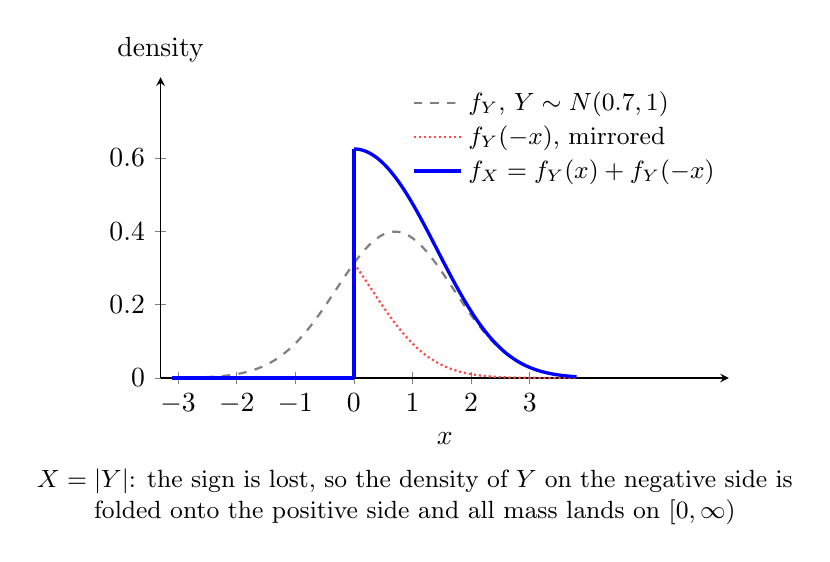
\begin{tikzpicture}
	\begin{axis}[
		axis lines=left, xmin=-3.3, xmax=6.4, ymin=0, ymax=0.82,
		xtick={-3,-2,-1,0,1,2,3}, ytick={0,0.2,0.4,0.6},
		xlabel={$x$}, ylabel={density}, ylabel style={rotate=-90, anchor=south, at={(axis description cs:0,1.02)}},
		samples=160, smooth, width=8.8cm, height=5.4cm, clip=false,
		legend style={draw=none, fill=none, font=\small, at={(1.0,0.99)}, anchor=north east}, legend cell align=left
		]
		\addplot[gray, thick, dashed, domain=-3.1:3.8] {exp(-(x-0.7)^2/2)/sqrt(2*pi)};
		\addlegendentry{$f_Y$, $Y\sim N(0.7,1)$}
		\addplot[red!70, thick, densely dotted, domain=0:3.8] {exp(-(x+0.7)^2/2)/sqrt(2*pi)};
		\addlegendentry{$f_Y(-x)$, mirrored}
		\addplot[blue, very thick, domain=0:3.8] {exp(-(x-0.7)^2/2)/sqrt(2*pi)+exp(-(x+0.7)^2/2)/sqrt(2*pi)};
		\addlegendentry{$f_X=f_Y(x)+f_Y(-x)$}
		\draw[blue, very thick] (axis cs:-3.1,0) -- (axis cs:0,0);
		\draw[blue, very thick] (axis cs:0,0) -- (axis cs:0,0.624);
	\end{axis}
	\node[anchor=north, font=\small, align=flush center, text width=9.6cm] at ([yshift=-2pt]current axis.outer south) {$X=|Y|$: the sign is lost, so the density of $Y$ on the negative side is folded onto the positive side and all mass lands on $[0,\infty)$};
\end{tikzpicture}
\end{document}
